\documentclass{extbook}[14pt]
\usepackage{multicol, enumerate, enumitem, hyperref, color, soul, setspace, parskip, fancyhdr, amssymb, amsthm, amsmath, bbm, latexsym, units, mathtools}
\everymath{\displaystyle}
\usepackage[headsep=0.5cm,headheight=0cm, left=1 in,right= 1 in,top= 1 in,bottom= 1 in]{geometry}
\pagestyle{fancy}
\lhead{}
\chead{Answer Key for Module\,6\,-\,Polynomial\,Functions Version A}
\rhead{}
\lfoot{Summer\,C\,2020}
\cfoot{}
\rfoot{}
\begin{document}
\textbf{This key should allow you to understand why you choose the option you did (beyond just getting a question right or wrong). \href{https://xronos.clas.ufl.edu/mac1105spring2020/courseDescriptionAndMisc/Exams/LearningFromResults}{More instructions on how to use this key can be found here}.}

\textbf{If you have a suggestion to make the keys better, \href{https://forms.gle/CZkbZmPbC9XALEE88}{please fill out the short survey here}.}

\textit{Note: This key is auto-generated and may contain issues and/or errors. The keys are reviewed after each exam to ensure grading is done accurately. If there are issues (like duplicate options), they are noted in the offline gradebook. The keys are a work-in-progress to give students as many resources to improve as possible.}

\rule{\textwidth}{0.4pt}

1. Describe the end behavior of the polynomial below.
\[ f(x) = -4(x - 9)^{2}(x + 9)^{5}(x - 6)^{2}(x + 6)^{4} \] 

 
 The solution is  
 \begin{center} 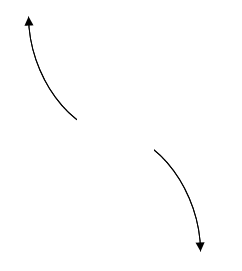
\includegraphics[width=0.3\textwidth]{../Figures/polyEndBehaviorAA.png} \end{center}\begin{tabular}{|c|c|} 
\hline 
 & \tabularnewline 
 \textbf{A.} 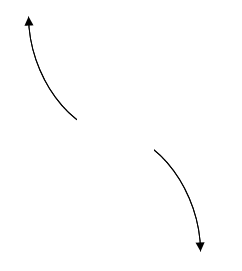
\includegraphics[width=0.3\textwidth]{../Figures/polyEndBehaviorAA.png} & \textbf{B.} 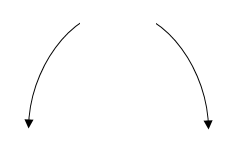
\includegraphics[width=0.3\textwidth]{../Figures/polyEndBehaviorBA.png} \tabularnewline 
\hline 
 & \tabularnewline 
 \textbf{C.} 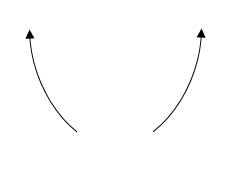
\includegraphics[width=0.3\textwidth]{../Figures/polyEndBehaviorCA.png} & \textbf{D.} 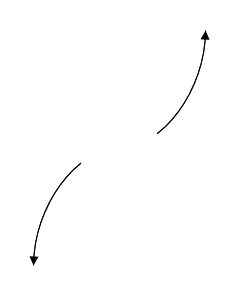
\includegraphics[width=0.3\textwidth]{../Figures/polyEndBehaviorDA.png} \tabularnewline 
\hline 
 E. None of the figures above. & \tabularnewline 
\hline 
 \end{tabular} 
 
\begin{enumerate}[label=\Alph*.] 
\item The function is above the $x$-axis, then passes through.  
\item The function is below the $x$-axis, then touches.  
\item The function is above the $x$-axis, then touches.  
\item The function is below the $x$-axis, then passes through.  
\end{enumerate} 
 
\textbf{General Comment:} \textbf{General Comments:} Remember that end behavior is determined by the leading coefficient AND whether the \textbf{sum} of the multiplicities is positive or negative. 

-----------------------------------------------

2. Construct the lowest-degree polynomial given the zeros below. Then, choose the intervals that contain the coefficients of the polynomial in the form $x^3+bx^2+cx+d$.
\[ -2 + 3 i \text{ and } x + 1 \] 
The solution is $ x^{3} +3 x^{2} +9 x -13 $ 

\begin{enumerate}[label=\Alph*.] 
\item $ b \in [-1.4, 2.7], c \in [-5.4, -1.8], \text{ and } d \in [-1, 11] $ 

 $x^{3} + x^{2} -4 x + 3$, which corresponds to multiplying out $(x -3)(x -1)$. 
\item $ b \in [-1.4, 2.7], c \in [-3.3, 4], \text{ and } d \in [-6, -1] $ 

 $x^{3} + x^{2} +x -2$, which corresponds to multiplying out $(x + 2)(x -1)$. 
\item $ b \in [-3.9, -0.8], c \in [8.2, 12.3], \text{ and } d \in [9, 21] $ 

 $x^{3} -3 x^{2} +9 x + 13$, which corresponds to multiplying out $(x-(-2 + 3 i))(x-(-2 - 3 i))(x + 1)$. 
\item $ b \in [2, 6.8], c \in [8.2, 12.3], \text{ and } d \in [-15, -10] $ 

 * $x^{3} +3 x^{2} +9 x -13$, which is the correct option. 
\item $ \text{None of the above.} $ 

 This corresponds to making an unanticipated error or not understanding how to use nonreal complex numbers to create the lowest-degree polynomial. If you chose this and are not sure what you did wrong, please contact the coordinator for help. 
\end{enumerate} 
 
\textbf{General Comment:} Remember that the conjugate of $a+bi$ is $a-bi$. Since these zeros always come in pairs, we need to multiply out $(x-(-2 + 3 i))(x-(-2 - 3 i))(x-(x + 1))$. 

-----------------------------------------------

3. Which of the following equations \textit{could} be of the graph presented below?
\begin{center} 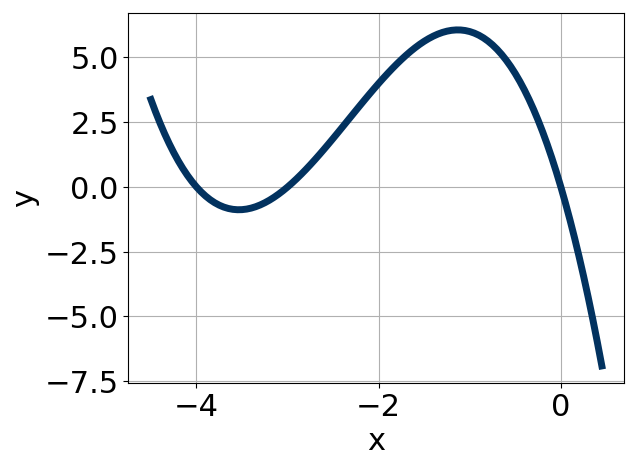
\includegraphics[width=0.3\textwidth]{../Figures/polyGraphToFunctionA.png} \end{center} 

The solution is $ -18x^{9} (x + 3)^{4} (x - 2)^{11} $ 

\begin{enumerate}[label=\Alph*.] 
\item $ 11x^{11} (x + 3)^{8} (x - 2)^{7} $ 

 This corresponds to the leading coefficient being the opposite value than it should be. 
\item $ -18x^{9} (x + 3)^{4} (x - 2)^{11} $ 

 * This is the correct option. 
\item $ -18x^{10} (x + 3)^{10} (x - 2)^{11} $ 

 The factor $x$ should have an odd power. 
\item $ 15x^{7} (x + 3)^{6} (x - 2)^{10} $ 

 The factor $(x - 2)$ should have an odd power and the leading coefficient should be the opposite sign. 
\item $ -11x^{6} (x + 3)^{9} (x - 2)^{5} $ 

 The factor $-3$ should have an even power and the factor $0$ should have an odd power. 
\end{enumerate} 
 
\textbf{General Comment:} General Comments: Draw the x-axis to determine which zeros are touching (and so have even multiplicity) or cross (and have odd multiplicity). 

-----------------------------------------------

4. Construct the lowest-degree polynomial given the zeros below. Then, choose the intervals that contain the coefficients of the polynomial in the form $ax^3+bx^2+cx+d$.
\[ \frac{4}{5}, \frac{3}{4}, \text{ and } \frac{3}{2} \] 
The solution is $ 40x^{3} -122 x^{2} +117 x -36 $ 

\begin{enumerate}[label=\Alph*.] 
\item $ a \in [37, 42], b \in [-131, -109], c \in [116, 124], \text{ and } d \in [-40, -34] $ 

 * $40x^{3} -122 x^{2} +117 x -36$, which is the correct option. 
\item $ a \in [37, 42], b \in [116, 124], c \in [116, 124], \text{ and } d \in [32, 40] $ 

 $40x^{3} +122 x^{2} +117 x + 36$, which corresponds to multiplying out $(5x + 4)(4x + 3)(2x + 3)$. 
\item $ a \in [37, 42], b \in [-131, -109], c \in [116, 124], \text{ and } d \in [32, 40] $ 

 $40x^{3} -122 x^{2} +117 x + 36$, which corresponds to multiplying everything correctly except the constant term. 
\item $ a \in [37, 42], b \in [-62, -57], c \in [-28, -24], \text{ and } d \in [32, 40] $ 

 $40x^{3} -58 x^{2} -27 x + 36$, which corresponds to multiplying out $(5x + 5)(4x -4)(2x -2)$. 
\item $ a \in [37, 42], b \in [-2, 6], c \in [-72, -67], \text{ and } d \in [-40, -34] $ 

 $40x^{3} +2 x^{2} -69 x -36$, which corresponds to multiplying out $(5x + 5)(4x + 4)(2x -2)$. 
\end{enumerate} 
 
\textbf{General Comment:} General Comments: To construct the lowest-degree polynomial, you want to multiply out $(5x -4)(4x -3)(2x -3)$ 

-----------------------------------------------

0. Describe the zero behavior of the zero $x = 9$ of the polynomial below.
\[ f(x) = 7(x + 9)^{4}(x - 9)^{7}(x + 6)^{7}(x - 6)^{8} \] 

 
 The solution is  
 \begin{center} 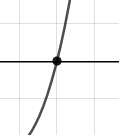
\includegraphics[width=0.3\textwidth]{../Figures/polyZeroBehaviorDA.png} \end{center}\begin{tabular}{|c|c|} 
\hline 
 & \tabularnewline 
 \textbf{A.} 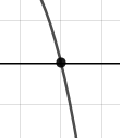
\includegraphics[width=0.3\textwidth]{../Figures/polyZeroBehaviorAA.png} & \textbf{B.} 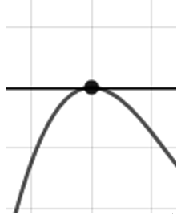
\includegraphics[width=0.3\textwidth]{../Figures/polyZeroBehaviorBA.png} \tabularnewline 
\hline 
 & \tabularnewline 
 \textbf{C.} 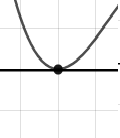
\includegraphics[width=0.3\textwidth]{../Figures/polyZeroBehaviorCA.png} & \textbf{D.} 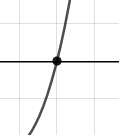
\includegraphics[width=0.3\textwidth]{../Figures/polyZeroBehaviorDA.png} \tabularnewline 
\hline 
 E. None of the figures above. & \tabularnewline 
\hline 
 \end{tabular} 
 
\begin{enumerate}[label=\Alph*.] 
\item   
\item   
\item   
\item   
\end{enumerate} 
 
\textbf{General Comment:} \textbf{General Comments:} You will need to sketch the entire graph, then zoom in on the zero the question asks about. 

-----------------------------------------------


\end{document}

